\section{Conditional GAN with projection discriminator}

So far, we have trained GANs that sample from a given dataset of images. However, many datasets come with not only images, 
but also labels that specify the class of that particular image. In the MNIST dataset, we have both the digit’s 
image as well as its numerical identity. It is natural to want to generate images that correspond to a particular class.

Formally, an \textit{unconditional} GAN is trained to produce samples $\bm{x} \sim p_{\theta}(\bm{x})$ that mimic samples 
$\bm{x} \sim p_{\text{data}}(\bm{x})$ from a data distribution. In the class-conditional setting, we instead have 
labeled data $(\bm{x}, y) \sim p_{\text{data}}(\bm{x}, y)$ and seek to train a model $p_{\theta}(\bm{x},y)$. 
Since it is the class conditional generator $p_{\theta}(\bm{x} \mid y)$ that we are interested in, we will express 
$p_{\theta}(\bm{x},y) = p_{\theta}(\bm{x} \mid y)p_{\theta}(y)$. We will set $p_{\theta}(\bm{x} \mid y)$ to be the distribution 
given by $G_{\theta}(\bm{z},y)$, where $\bm{z} \sim \calN(0,I)$ as usual. For simplicity, we will assume 
$p_{\text{data}}(y) = \frac{1}{m}$ and set $p_{\theta}(y) = \frac{1}{m}$, where $m$ is the number of classes. 
In this case, the discriminator’s loss becomes

\begin{equation} \label{eq:17}
    L_D(\phi; \theta) = - \E_{(\bm{x}, y) \sim p_{\text{data}}(\bm{x}, y)}[\log D_{\phi}(\bm{x}, y)] - \E_{(\bm{x},y) \sim p_{\theta}(\bm{x},y)}[\log (1 - D_{\phi}(\bm{x},y))]
\end{equation}

\begin{equation} \label{eq:18}
   = - \E_{(\bm{x}, y) \sim p_{\text{data}}(\bm{x}, y)}[\log D_{\phi}(\bm{x}, y)] - \E_{y \sim p_{\theta}(y)}[ \E_{\bm{z} \sim \calN(0,I)}[ \log (1 - D_{\phi}(G_{\theta}(\bm{z}, y), y))]]
\end{equation}

Therefore, the main difference for the conditional GAN is that we must structure our generator $G_{\theta}(\bm{z},y)$ 
and discriminator $D_{\phi}(\bm{x}, y)$ to accept the class label $y$ as well. For the generator, one simple way to do 
so is to encode $y$ as a one-hot vector $\bm{y}$ and concatenate it to $\bm{z}$, and then apply neural network layers normally. 
(A one-hot representation of a class label $y$ is an $m$-dimensional vector $\bm{y}$ that is 1 in the $y$th entry and 0 
everywhere else.) 

In practice, the effectiveness of the model is strongly dependent on the way the discriminator depends on $y$. 
One heuristic with which to design the discriminator is to mimic the form of the theoretically optimal discriminator. 
That is, we can structure the neural network used to model $D_{\phi}$ based on the form of $D^{*}$, where $D^{*}$ minimizes $L_D$. 
To calculate the theoretically optimal discriminator, though, it is necessary to make some assumptions.

\begin{enumerate}[label=(\alph*)]
    \item \input{04-cgan/01-simplify}

    \item \points{4b} Implement and train a conditional GAN on Fashion MNIST for one epoch. The discriminator has the structure 
    described in part 4\label{4a}, with $\varphi$, $A$ and $b$ parameterized by a neural network with a final linear layer, 
    and the generator accepts a one-hot encoding of the class. In \texttt{submission/gan.py}, implement the 
    \texttt{conditional\_loss\_nonsaturating\_g} and \texttt{conditional\_loss\_nonsaturating\_d} functions. 
    
    To train the model, execute:
    \begin{verbatim}
        python main.py --model cgan --out_dir gan_nonsat_conditional
    \end{verbatim} 

    For GPU acceleration run run the command below. \textbf{Note:} we are not supporting MPS GPUs as it trains slower than CPU-enabled training on Apple Silicon devices.
    \begin{verbatim}
        python main.py --model cgan --out_dir gan_nonsat_conditional --device gpu
    \end{verbatim} 

    You may monitor the GAN's output in 
    the \texttt{gan\_nonsat\_conditional} directory. You should be able to roughly recognize the 
    categories that correspond to each column. The final image generated after training should resemble the following image below:

    For reference, the generated examples should look similar to the image below:
    \begin{figure}[h]
        \centering
        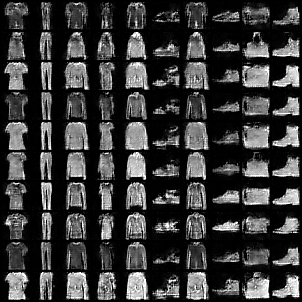
\includegraphics[width=0.5\textwidth]{./figures/cgan_nonsat_0900}
    \end{figure}

\end{enumerate}